\documentclass[9pt,twocolumn,twoside,lineno]{pnas-new}
\usepackage{bm,bbm}
\usepackage{nicefrac}
\usepackage{amsmath}
% Use the lineno option to display guide line numbers if required.
%\usepackage{scalerel}
\usepackage{booktabs}       % professional-quality tables
\usepackage{nicefrac}       % compact symbols for 1/2, etc.
\usepackage{amsmath}
\usepackage{amsthm}
\usepackage{amssymb}
\usepackage{amsfonts}
\usepackage{mathtools}
\usepackage{amsmath}
\usepackage{txfonts}

\usepackage{fontawesome}

\newtheorem{assumption}{Assumption}
\newtheorem{corollary}{Corollary}
\newtheorem{problem*}{Problem}
\newtheorem{property}{Property}
\newtheorem{theorem}{Theorem}
\newtheorem{lemma}{Lemma}
\newtheorem{remark}{Remark}
\newtheorem{definition}{Definition}
\newtheorem{proposition}{Proposition}
\newtheorem{claim}{Claim}
\newtheorem{example}{Example}
\newtheorem*{example*}{Example}

\usepackage[ruled,linesnumbered,noresetcount,vlined]{algorithm2e}
\makeatletter
\newcommand{\nlsetend}[1]{%
\SetKwIF{nlIf}{ElseIf}{Else}{if}{then}{else if}{else}{\nlset{#1}end}
}
\newcommand{\nosemic}{\renewcommand{\@endalgocfline}{\relax}}% Drop semi-colon ;
\newcommand{\dosemic}{\renewcommand{\@endalgocfline}{\algocf@endline}}% Reinstate semi-colon ;
\newcommand{\pushline}{\Indp}% Indent
\newcommand{\popline}{\Indm\dosemic}% Undent
\let\oldnl\nl% Store \nl in \oldnl
\newcommand{\nonl}{\renewcommand{\nl}{\let\nl\oldnl}}% Remove line number for one line
\renewcommand\AlCapNameSty{\slshape}
\SetKwFor{Repeat}{repeat}{:}{endw}
\makeatother
\usepackage{todonotes}
\usepackage{xcolor}
\usepackage{setspace}
\usepackage{multirow}
\usepackage{bm,bbm}
\usepackage{paralist}
\usepackage{enumitem}

\newcommand{\Lap}{\textrm{Lap}}
\DeclareMathOperator*{\argmax}{argmax}
\DeclareMathOperator*{\argmin}{argmin}
\DeclareMathOperator*{\minimize}{minimize}
\newcommand*{\prob}{\mathsf{P}}

%%% Comments
\newcommand{\nandoSide}[1]{\todo[caption={},color=cyan!20!]{
\begin{spacing}{0.6}
\vspace{-2pt}
{\tiny FF: #1}
\vspace{-8pt}
\end{spacing}}}
\newcommand{\pascalSide}[1]{\todo[caption={},color=green!20!]{
\begin{spacing}{0.6}
\vspace{-2pt}
{\tiny PVH: #1}
\vspace{-8pt}
\end{spacing}}}
\newcommand{\cuongSide}[1]{\todo[caption={},color=red!20!]{
\begin{spacing}{0.6}
\vspace{-2pt}
{\tiny CT: #1}
\vspace{-8pt}
\end{spacing}}}
\newcommand{\nando}[1]{\todo[inline,caption={},color=cyan!20!]{
\begin{spacing}{0.6}
\vspace{-2pt}
{\footnotesize FF: #1}
\vspace{-8pt}
\end{spacing}}}
\newcommand{\cuong}[1]{\textbf{CT}:{\color{red}{#1}}}


\definecolor{darkgreen}{RGB}{204,102,0}

\newcommand{\rev}[1]{{\color{purple}{#1}}}
\newcommand{\add}[1]{{\color{darkgreen}{#1}}}
\newcommand*{\defeq}{\stackrel{\text{def}}{=}}
\def\aux{\mathrm{aux}}

% Math-cal
\newcommand{\cA}{\mathcal{A}} \newcommand{\cB}{\mathcal{B}} 
\newcommand{\cC}{\mathcal{C}} \newcommand{\cD}{\mathcal{D}}
\newcommand{\cE}{\mathcal{E}} \newcommand{\cF}{\mathcal{F}}
\newcommand{\cG}{\mathcal{G}} \newcommand{\cH}{\mathcal{H}}
\newcommand{\cI}{\mathcal{I}} \newcommand{\cL}{\mathcal{L}}
\newcommand{\cM}{\mathcal{M}} \newcommand{\cN}{\mathcal{N}}
\newcommand{\cO}{\mathcal{O}} \newcommand{\cP}{\mathcal{P}}
\newcommand{\cR}{\mathcal{R}} \newcommand{\cS}{\mathcal{S}}
\newcommand{\cT}{\mathcal{T}} \newcommand{\cV}{\mathcal{V}}
\newcommand{\cZ}{\mathcal{Z}} \newcommand{\cJ}{\mathcal{J}}
\newcommand{\cK}{\mathcal{K}} \newcommand{\cY}{\mathcal{Y}}
\newcommand{\cW}{\mathcal{W}} \newcommand{\cX}{\mathcal{X}}

\newcommand{\EE}{\mathbb{E}} \newcommand{\RR}{\mathbb{R}}
\newcommand{\NN}{\mathbb{N}} \newcommand{\ZZ}{{\mathbb{Z}}}
\newcommand{\CC}{{\mathbb{C}}}

%%% helpers
\newcommand{\MLap}{\mathcal{M}_{\mathrm{Lap}}}
\newcommand{\var}{\mathrm{Var}}
\newcommand{\cov}{\mathrm{Cov}}

\newcommand{\minimize}[1]{\underset{{#1}}{\text{minimize}}}
\newcommand{\maximize}[1]{\underset{{#1}}{\text{maximize}}}
% \newcommand{\st}{\text{subject to}}
\newcommand{\setcard}[1]{\scalebox{0.5}{$|#1|$}}
% \usepackage{mathtools}
\newcommand\norm[1]{\left\lVert#1\right\rVert}
\usepackage{esvect}\newcommand{\cev}[1]{\reflectbox{\ensuremath{\vec{\reflectbox{\ensuremath{#1}}}}}}
\DeclareMathOperator{\Tr}{Tr}
\newcommand{\se}[1]{\text{s}(#1)}
\newcommand{\re}[1]{\text{r}(#1)}
\newcommand{\ra}[1]{\renewcommand{\arraystretch}{#1}}
\newcommand{\smallk}{\scalebox{0.65}{$k$}}
\newcommand{\userset}{\cP}
\newcommand{\unitset}{\cU}
\newcommand{\regionset}{\cR}
\newcommand{\unitsizeset}{\cZ}
\newcommand{\sizeset}{\cS}
\newcommand{\user}{p}
% \newcommand{\unit}{u}
% \newcommand{\region}{r}
\newcommand{\unitsize}{z}
\newcommand{\size}{\sigma}
\newcommand{\group}{G}
\newcommand{\gsize}{n}
\newcommand{\gsizevec}{\bm{n}}
\newcommand{\csize}{c}
\newcommand{\csizevec}{\bm{c}}

\newcommand{\node}{a}
\newcommand{\US}{\textsl{US}}
\newcommand{\GA}{\textsl{GA}}
\newcommand{\MI}{\textsl{MI}}
\newcommand{\ctable}{\bm{\tau}}
\newcommand{\cfunction}{\mathring{\ctable}}
\newcommand{\ctablech}{\bm{\phi}}
\newcommand{\cfunctionch}{\mathring{\ctablech}}

\newcommand{\dom}{D}
\newcommand{\tree}{\cT}
\newcommand{\treedp}{\cT^{\textsl{dp}}}
\DeclareMathOperator{\Tr}{Tr}
\DeclarePairedDelimiter\ceil{\lceil}{\rceil}
\DeclarePairedDelimiter\floor{\lfloor}{\rfloor}
\DeclarePairedDelimiter{\nint}\lfloor\rceil

%%% KEYU NOTATIONS 

\newcommand{\bB}{\mathbf{B}}
\newcommand{\bD}{\mathbf{D}}
\newcommand{\bE}{\mathbf{E}}
\newcommand{\bF}{\mathbf{F}}
\newcommand{\bG}{\mathbf{G}}
\newcommand{\bL}{\mathbf{L}}
\newcommand{\bT}{\mathbf{T}}
\newcommand{\bX}{\setf{X}}
\newcommand{\bY}{\setf{Y}}
\newcommand{\bv}{\setf{v}}
\newcommand{\bj}{\setf{j}}
\newcommand{\bn}{\setf{n}}

\newcommand{\bc}{\mathbf{c}}
\newcommand{\bg}{\mathbf{g}}

\newcommand{\bs}{\bm{\sigma}}
\newcommand{\bS}{\bm{\Sigma}}

\newcommand{\bx}{\mathbf{x}}
\newcommand{\bw}{\setf{w}}
\newcommand{\bz}{\setf{z}}
\newcommand{\xl}{\mathbf{x}_{\ell}}
\newcommand{\xg}{\mathbf{x}_{g}}


% Math-scr
\newcommand{\sU}{{\mathscr{U}}}	% a subset of  therange of the databases
\newcommand{\sF}{{\mathscr{F}}} % collections of features
\newcommand{\sR}{{\mathscr{R}}}


\newcommand{\M}{{\mathcal{M}}}
\newcommand{\x}{D_1}
\newcommand{\y}{D_2}
\newcommand{\private}[1]{\tilde{#1}}
\newcommand{\data}{D}
\newcommand{\D}{{\mathscr{D}}}	% the set of all databases
\newcommand{\sD}{{\mathscr{D}}}	% the set of all databases
\newcommand{\R}{{\mathscr{R}}}	% the range of all databases
\newcommand{\s}{{\mathcal{S}}}	% a subset of the range of the 
\newcommand{\sO}{{\mathscr{O}}}	% the set of all databases


\newcommand{\X}{{\mathcal{X}}}
\newcommand{\Mode}{\setf{M}}
\newcommand{\sd}{\setf{d}}
\newcommand{\MLap}{\mathcal{M}_{\mathrm{Lap}}}
\newcommand{\FQ}{FQ}


\newcommand{\Lap}{{\text{Lap}}}
\newcommand{\q}[1]{c_{#1}}
\newcommand{\nq}[1]{\tilde{c}_{#1}}
\newcommand{\h}[1]{h_{#1}}
\newcommand{\nh}[1]{\tilde{h}_{#1}}
\newcommand{\projod}[1]{\data_{|\setf{L}\!=\!{#1}}}
\newcommand{\isin}{\!\in\!}
\newcommand{\isto}{\!\to\!}
\newcommand{\isst}{\!:\!}
\newcommand{\cmark}{\ding{51}}%
\newcommand{\xmark}{\ding{55}}%

\newcommand{\triplet}{triplet\xspace}
\newcommand{\triplets}{triplets\xspace}
\newcommand{\featurespec}{feature specification\xspace}
\newcommand{\OBM}{CBDP\xspace}
\newcommand{\MO}{\M_{O}\xspace}
\newcommand{\MOi}[1]{\M_{O#1}}
\newcommand{\nth}[1]{$#1^\text{th}$}
\def \algname{\textsc{OptStream}}

\newcommand*{\skipnumber}[2][1]{%
   {\renewcommand*{\alglinenumber}[1]{}\State #2}%
   \addtocounter{ALG@line}{-#1}}
\def \iff{\;\Leftrightarrow\;}

%--------------------------------------------------------------------
%	ENVIRONMENTS: ITEMIZE 
%--------------------------------------------------------------------
\newcommand{\benumerate}{\begin{list}{$\bullet$}{\topsep=0pt \parsep=0pt \itemsep=1pt \labelwidth=1.5em \labelsep=0.5em \leftmargin=20pt}}
\newcommand{\eenumerate}{\end{list}}
\newcommand{\bitemize}{\begin{list}{$\bullet$}{\topsep=0pt \parsep=0pt \itemsep=0pt \leftmargin=10pt}}
\newcommand{\eitemize}{\end{list}}

\newcommand{\iOne}{\textit{(i)}\xspace}
\newcommand{\iTwo}{\textit{(ii)}\xspace}
\newcommand{\iThree}{\textit{(iii)}\xspace}
\newcommand{\iFour}{\textit{(iv)}\xspace}
\newcommand{\iFive}{\textit{(v)}\xspace}

%--------------------------------------------------------------------
%	ENVIRONMENTS: Comments
%--------------------------------------------------------------------
\newcommand{\nandoSide}[1]{\todo[caption={},color=blue!20!]{{\footnotesize Nando: #1}}}
\newcommand{\nando}[1]{\todo[inline,caption={},color=blue!20!]{Nando: #1}}

\newcommand{\pascalSide}[1]{\todo[caption={},color=red!20!]{{\footnotesize Pascal: #1}}}
\newcommand{\pascal}[1]{\todo[inline,caption={},color=red!20!]{Pascal: #1}}


%	ENVIRONMENTS: FLOATS: tables and figures 
\def\emptycell{\multicolumn{1}{c}{}}
%	COMMANDS: MATH
\newcommand{\tuple}[1]{\langle #1 \rangle}
\newcommand{\andl}{\hspace{3pt} \land \hspace{3pt}}
\newcommand{\bigO}[1]{$O\big(#1\big)$}
\newcommand{\bigo}[1]{\small{O\big(#1\big)}}
\def\is{\!=\!}
\def\st{\: | \:}
\def\oof{\:\mathbf{of} \:\:}
\newcommand{\argmax}{\operatornamewithlimits{argmax}}
\newcommand{\argmin}{\operatornamewithlimits{argmin}}
\newcommand{\minimize}{\operatornamewithlimits{minimize}}
\newcommand{\argminmax}{\operatornamewithlimits{arg \min\!/\!\max}}
\newcommand{\argprec}{\operatornamewithlimits{arg\!\prec}}
%\DeclareMathOperator*{\bigtimes}{\vartimes}
\newcommand{\scope}[1]{\setf{x}^{#1}}
% COMMANDS: FONTS
\newcommand{\listf}[1]{{\mathcal{#1}}}
\newcommand{\setf}[1]{{\bf{#1}}}
\newcommand{\res}[1]{\bm{\Delta}\left(#1\right)}
\newcommand{\varf}[1]{{\it{#1}}}
\newcommand{\parsection}[1]{\vspace{8pt}\noindent\textbf{\textit{\underline{#1}}}.\hspace{8pt}\noindent}
\newcommand{\algref}[2]{\medskip\noindent\textbf{#1} \cite{#2}.\hspace{4pt}}
\newcommand{\domainref}[1]{\medskip\noindent\textbf{#1}.\hspace{4pt}}
\newcommand{\highlight}[1]{\underline{\textit{#1}}}


\DeclarePairedDelimiter\ceil{\lceil}{\rceil}
\DeclarePairedDelimiter\floor{\lfloor}{\rfloor}
\DeclarePairedDelimiter{\nint}\lfloor\rceil
\templatetype{pnasresearcharticle} % Choose template 
% {pnasresearcharticle} = Template for a two-column research article
% {pnasmathematics} %= Template for a one-column mathematics article
% {pnasinvited} %= Template for a PNAS invited submission

\newtheorem{definition}{Definition}
\newcommand{\cW}{\mathcal{W}}
\newcommand{\cM}{\mathcal{M}}
\newcommand{\cR}{\mathcal{R}}
\newcommand{\cX}{\mathcal{X}}
\newcommand{\EE}{\mathbb{E}} \newcommand{\RR}{\mathbb{R}}
\newcommand{\NN}{\mathbb{N}} \newcommand{\ZZ}{{\mathbb{Z}}}
\newcommand{\CC}{{\mathbb{C}}}
\newcommand{\truedata}{\bm{x}}
\newcommand{\weight}{\bm{a}}
\newcommand{\truealloc}{\alloc{\truedata}}
\newcommand{\noisyalloc}{\alloc{\noisydata}}
\newcommand{\noisydata}{\tilde{\bm{x}}}

\newcommand{\norm}[1]{\left\lVert#1\right\rVert}

\newtheorem{assumption}{Assumption}
\newtheorem{corollary}{Corollary}
\newtheorem{problem*}{Problem}
\newtheorem{property}{Property}
\newtheorem{theorem}{Theorem}
\newtheorem{lemma}{Lemma}
\newtheorem{remark}{Remark}
\newtheorem{proposition}{Proposition}
\newtheorem{claim}{Claim}
\newtheorem{example}{Example}

 \usepackage{pstricks}
    
    

    \newcommand{\diff}[1]{\bm{d}\left(#1\right)}
    \newcommand{\col}[1]{\operatorname{col}\left(#1\right)}
    \newcommand{\row}[1]{\operatorname{row}\left(#1\right)}
    \newcommand{\rank}[1]{\operatorname{rank}\left(#1\right)}
    \newcommand{\tr}[1]{\operatorname{tr}\left(#1\right)}
    \newcommand{\cov}[1]{\operatorname{Cov}\left(#1\right)}
    \newcommand{\lspan}[1]{\operatorname{span}\left(#1\right)}
    
    \newcommand{\bias}[2]{\operatorname{Bias}\left(#1,#2\right)}
    \newcommand{\diserr}[2]{\xi\left(#1,#2\right)}
    \newcommand{\pr}[1]{\operatorname{Pr}\left(#1\right)}
    \newcommand{\var}[1]{\operatorname{Var}\left(#1\right)}
    \newcommand{\inner}[2]{\left\langle#1,#2\right\rangle}
    \newcommand{\vecangle}[2]{\angle\left(#1,#2\right)}
    \newcommand{\err}[1]{\operatorname{Err}\left(#1\right)}
    \newcommand{\proj}[2]{\Pi_{#1}\left(#2\right)}
    \newcommand{\BB}[2]{B_{#1}\left(#2\right)}
    \newcommand{\opt}[1]{\operatorname{Opt}\left(#1\right)}
    \newcommand{\relu}[1]{\left(#1\right)_+}
    \newcommand{\alloc}[1]{P^F\left(#1\right)}
     \newcommand{\blmech}[1]{\cM_{\mathrm{BL}}\left(#1\right)}
    \newcommand{\posmech}[1]{\cM_{\mathrm{PoS}}\left(#1\right)}
    \newcommand{\andmech}[1]{\cM_{\mathrm{A\&D}}\left(#1\right)}
    \newcommand{\pamech}[1]{\cM_{\mathrm{PA}}\left(#1\right)}
    \newcommand{\rpmech}[1]{\cM_{\mathrm{RP}}\left(#1\right)}
    \newcommand{\talloci}[1]{P^F_{#1}\left(\truedata\right)}
    \newcommand{\nalloci}[1]{P^F_{#1}\left(\noisydata\right)}
    
    

   
    
    \newcommand{\unit}{\bm{e}}
    \newcommand{\newunit}{\bm{e}'}
    
    \newcommand{\refopt}{\operatorname{Ref}}
    % \newcommand{\supp}{\operatorname{supp}}
    \newcommand{\noise}{\bm{\eta}}
    \newcommand{\cop}{B^+}
    \newcommand{\radius}{r_m}

    
    \newcommand{\cN}{{\mathcal{N}}}
    \newcommand{\cI}{{\mathcal{I}}}
    \newcommand{\cJ}{{\mathcal{J}}}
    \newcommand{\chat}{\hat{\bm{c}}}
    \newcommand{\dhat}{\hat{\bm{d}}}
    

\title{Bias in allocations using differentially private census data: An analysis of the 2020 U.S.~Census}

% Use letters for affiliations, numbers to show equal authorship (if applicable) and to indicate the corresponding author
\author[a,c,1]{Author One}
\author[b,1,2]{Author Two} 
\author[a]{Author Three}

\affil[a]{Affiliation One}
\affil[b]{Affiliation Two}
\affil[c]{Affiliation Three}

% Please give the surname of the lead author for the running footer
\leadauthor{Lead author last name} 

% Please add a significance statement to explain the relevance of your work
\significancestatement{Authors must submit a 120-word maximum statement about the significance of their research paper written at a level understandable to an undergraduate educated scientist outside their field of speciality. The primary goal of the significance statement is to explain the relevance of the work in broad context to a broad readership. The significance statement appears in the paper itself and is required for all research papers.}

% Please include corresponding author, author contribution and author declaration information
\authorcontributions{Please provide details of author contributions here.}
\authordeclaration{Please declare any competing interests here.}
\equalauthors{\textsuperscript{1}A.O.(Author One) contributed equally to this work with A.T. (Author Two) (remove if not applicable).}
\correspondingauthor{\textsuperscript{2}To whom correspondence should be addressed. E-mail: author.two\@email.com}

% At least three keywords are required at submission. Please provide three to five keywords, separated by the pipe symbol.
\keywords{Keyword 1 $|$ Keyword 2 $|$ Keyword 3 $|$ ...} 

\begin{abstract}
% Agencies, such as the U.S. Census Bureau, release data  sets  and  statistics  about  groups  of  individuals  that  are  used  as  input  to  a  number  of  critical decision processes.   To conform with privacy and confidentiality requirements, these agencies are of-ten required to release privacy-preserving versions of the data.   This paper studies the release of differentially private data sets and analyzes their impact on some critical resource allocation tasks under a fairness perspective.   The paper shows that,when the decisions take as input differentially private data,  the noise added to achieve privacy dis-proportionately impacts some groups over others.The paper analyzes the reasons for these disproportionate impacts and proposes guidelines to mitigate these effects.  The proposed approaches are evaluated on critical decision problems that use differentially private census data
The decennial census is a primary source of data for the US government to make critical decisions. For example,  132 programs used Census Bureau data to distribute more than \$675 billion in funds during fiscal year 2015. In order to ensure the published census data does not reveal individual information, the Census Bureau adopts the differential privacy (DP) technique. In particular, in 2020, the Census Bureau implemented the Top Down algorithm which release statistical data from top (nation) to bottom hierarchical level (block). However, it was recently observed that the DP outcomes can introduce biased outcomes, especially for minority groups. In this paper, we analyze the reasons for these disproportionate impacts and proposes guidelines to mitigate these effects. We focus on two aspects that can produce the fair outcomes: (1) shape of allocation function and (2) impact of post-processing steps. 
\end{abstract}

\dates{This manuscript was compiled on \today}
\doi{\url{www.pnas.org/cgi/doi/10.1073/pnas.XXXXXXXXXX}}

\begin{document}

\maketitle
\thispagestyle{firststyle}
\ifthenelse{\boolean{shortarticle}}{\ifthenelse{\boolean{singlecolumn}}{\abscontentformatted}{\abscontent}}{}



% If your first paragraph (i.e. with the \dropcap) contains a list environment (quote, quotation, theorem, definition, enumerate, itemize...), the line after the list may have some extra indentation. If this is the case, add \parshape=0 to the end of the list environment.
% \dropcap{T}his PNAS journal template is provided to help you write your work in the correct journal format. Instructions for use are provided below. 

% Note: please start your introduction without including the word ``Introduction'' as a section heading (except for math articles in the Physical Sciences section); this heading is implied in the first paragraphs. 
\section*{Introduction}

Agencies, such as the U.S.~Census Bureau, release data sets and
statistics about groups of individuals that are then used as inputs to
a number critical decision processes.  For example, the census data is
used to decide whether a jurisdiction must provide language assistance
during elections, Title I fund allocation in education \cite{pujol:20}
and to establish national level COVID-19 vaccination distribution plans 
for states and jurisdictions \cite{covid}.
The resulting decisions can have significant societal, economic, and medical 
consequences for participating individuals. 

In many cases, the released data
contain sensitive information and their privacy is strictly regulated.
For example, in the U.S., the census data is regulated under Title 13
\cite{title13}, which requires that no individual be identified from
any data release by the Census Bureau. In Europe, data release are
regulated according to the \emph{General Data Protection Regulation}
\cite{GDPR}, which addresses the control and transfer of personal data.

Statistical agencies thus release \emph{privacy-preserving} data and
statistics that conform to privacy and confidentiality requirements.
In the U.S., a small number of decisions, such as congressional
apportionment, are taken using unprotected true values, but the vast
majority of decisions rely on privacy-preserving data. Of particular
interest are resource allocation decisions relying on the U.S.~Census
Bureau data, since the bureau will release several privacy-preserving 
data products using the framework of \emph{Differential Privacy} \cite{abowd2018us}
for their 2020 release. In particular, in  2020 the Census Bureau implemented a new privacy preserving framework to release privately hierarchical statistical data, the Top Down algorithm. The algorithms works by firstly splitting the given privacy budget $\epsilon$ to six hierarchical levels (nation, state, county, tract, block, group—block). Then in the second step, a post-processing step is applied to make sure the noisy counts are consistent, e.g., the counts should be non-negative. 
However, \cite{pujol:20} empirically showed
that differential privacy may have a disparate impact on several
resource allocation problems. The noise introduced by the privacy
mechanism may result in decisions that impact various groups
differently. Unfortunately, the paper did not provide a deep understanding why this behavior happens and any mitigation to resolve the issue. This paper builds on these observations and provides a step towards a
deeper understanding of the fairness issues arising when
differentially private data is used as input to several resource
allocation problems.  {\em One of its main results is to prove that
  several allotment problems and decision rules with significant
  societal impact (e.g., the allocation of educational funds, the
  decision to provide minority language assistance on election
  ballots, or the distribution of COVID-19 vaccines) exhibit inherent
  unfairness when applied to a differentially private release of the census
  data.} To counteract this negative results, the paper examines the
conditions under which decision making is fair when using differential
privacy, and techniques to bound unfairness. The paper also provides a
number of mitigation approaches to alleviate biases introduced by
differential privacy on such decision making problems. More
specifically, the paper makes the following contributions:
\begin{enumerate}[leftmargin=*,labelsep=2pt,itemsep=0pt,parsep=2pt,topsep=2pt]

\item It formally defines notions of fairness and bounded fairness for decision making
  subject to privacy requirements. 

\item It examines the roots of the induced unfairness by analyzing the structure
  of the decision making problems. 

\item It proposes several guidelines to mitigate the negative
  fairness effects of the decision problems studied.  
\end{enumerate}

To the best of the authors' knowledge, this is the first study that
attempt at characterizing the relation between differential privacy
and fairness in decision problems. All proofs are reported in the
appendix. [Is this still true?]

%%%%%%%%%%%%%%%%%%%%%%%%%%%%%%%%%%%%%%

\section*{Preliminaries: Differential Privacy}
%%%%%%%%%%%%%%%%%%%%%%%%%%%%%%%%%%%%%%%%%%%%%%%%%%%%%%%%%%%%%%%%%%%%%

\emph{Differential Privacy} \cite{Dwork:06} (DP) is a rigorous privacy notion that characterizes the amount of information of an individual's data being disclosed in a computation.


\begin{definition}%[Differential Privacy \cite{Dwork:06}]
  A randomized algorithm $\cM:\cX \to \cR$ with domain $\cX$ and range $\cR$ satisfies $\epsilon$-\emph{differential privacy} if
  for any output $O \subseteq \cR$ and data sets $\bm{x}, \bm{x}' \in \cX$ differing by at most one entry (written $\bm{x} \sim \bm{x}'$) 
  \begin{equation}
  \label{eq:dp}
    \Pr[\cM(\bm{x}) \in O] \leq \exp(\epsilon) \Pr[\cM(\bm{x}') \in O]. 
  \end{equation}
\end{definition}

\noindent 
Parameter $\epsilon \!>\! 0$ is the \emph{privacy loss}, with values close 
to $0$ denoting strong privacy. Intuitively, DP states that 
any event occur with similar probability regardless of the participation
of any individual data to the data set. 

DP satisfies several properties including 
\emph{immunity to post-processing}, which states that the privacy 
loss of DP outputs is not affected by arbitrary data-independent 
post-processing \cite{Dwork:13}.

A function $f$ from a data set $\bm{x} \in \cX$ to a result set 
$R \subseteq \RR^n$ can be made differentially private by injecting 
random noise onto its output. The amount of noise relies on the notion 
of \emph{global sensitivity} %, denoted by $\Delta_f$ and defined as
\(
\Delta_f = \max_{\bm{x} \sim \bm{x}'} \| f(\bm{x}) - f(\bm{x}') \|_1.
\)
The \emph{Laplace mechanism} \cite{Dwork:06} that outputs $f(\bm{x}) + \bm{\eta}$, where $\bm{\eta} \in \RR^n$ is drawn from the i.i.d.~Laplace distribution with $0$ mean and scale  $\nicefrac{\Delta_f}{\epsilon}$ over $n$ dimensions, achieves $\epsilon$-DP. Similarly, once can also utilize the Gaussian mechanism to satisfy $\epsilon$-DP by sampling from the Gaussian distribution with mean 0 and scale $\nicefrac{\Delta_f}{\epsilon}$. 

%%%%%%%%%%%%%%%%%%%%%%%%%%%%%%%%%%%%%%%%%%%%%%%%%%%%%%%%%%%%%%%%%%%%%
\section*{Problem Setting and Goals}
\label{sec:setting}
%%%%%%%%%%%%%%%%%%%%%%%%%%%%%%%%%%%%%%%%%%%%%%%%%%%%%%%%%%%%%%%%%%%%%


The paper considers a dataset $\bm{x} \!\in\! \cX \subseteq \RR^k$ of $n$ entities, 
whose elements $x_i= (x_{i1},\ldots, x_{1k})$ describe $k$ measurable 
quantities of entity $i \!\in\! [n]$, such as the number of individuals living 
in a geographical region $i$ and their English proficiency. 
The paper considers two classes of problems: 
\begin{itemize}[leftmargin=*,labelsep=2pt,itemsep=0pt,parsep=2pt,topsep=2pt]
\item An \emph{allotment problem} $P : \cX \times [n] \to \mathbb{R}$ is a function that distributes a finite set of resources to some problem entity. $P$ may represent, for instance, the amount of money allotted to a school district. 
\item A \emph{decision rule} $P: \cX \times [n] \to \{0,1\}$
  determines whether some entity qualifies for some benefits.  For
  instance, $P$ may represent if election ballots should be described
  in a minority language for an electoral district.
% https://www.justice.gov/crt/about-language-minority-voting-rights
\end{itemize}
The paper assumes that $P$ has bounded range, and uses the shorthand
$P_i(\bm{x})$ to denote $P(\bm{x}, i)$ for entity $i$.
%
The focus of the paper is to study the effects of a DP data-release
mechanism $\cM$ to the outcomes of problem $P$. Mechanism $\cM$ is
applied to the dataset $\bm{x}$ to produce a privacy-preserving
counterpart $\tilde{\bm{x}}$ and the resulting private outcome
$P_i(\tilde{\bm{x}})$ is used to make some allocation decisions.

\begin{figure}[!t] 
\centering
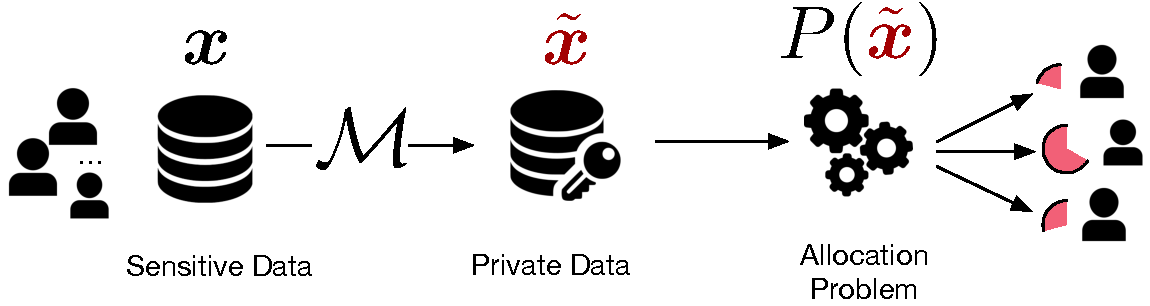
\includegraphics[width=0.9\columnwidth]{images/figure.pdf}
\caption{Diagram of the private allocation problem.}
\label{fig:framework}
\end{figure}
Figure \ref{fig:framework} provides an illustrative diagram. 

Because random noise is added to the original dataset $\bm{x}$, the output $P_i(\tilde{\bm{x}})$ incurs some error. {\em The focus of this paper is to characterize and quantify the disparate impact of this error among the problem entities}. In particular, the paper focuses on two notations of errors. 

\begin{definition}[Statistical bias]
\label{def:bias}
The statistical bias  $ B_P^i(\cM, \bm{x}) $ of the mechanism $\cM$ measures the difference between the expected private outcome with the true outcome: 
 \begin{equation}
 \label{eq:bias}
  B_P^i(\cM, \bm{x}) = 
  %\left| 
  \EE_{\tilde{\bm{x}} \sim \cM(\bm{x})} \left[ P_i(\tilde{\bm{x}}) \right] - P_i (\bm{x}),
  %\right|,
   \end{equation}

\end{definition}

The paper also considers another notation of error which is the normalized version of the above bias.
\begin{definition}[Multiplicative error]
The multiplicative error under mechanism $\cM$ and problem $P$ for entity $i$ is given by: $\nicefrac{B_P^i(\cM, \bm{x})}{P^i(x)}$

\end{definition}

Our notion of fairness will be based on these two notations of errors. 


\begin{definition}[$\alpha$-fairness \cite{fioretto2021decision}]
        Given the true data $\truedata$, the mechanism $\cM$ is said to be \emph{$\alpha$-fair} if, for any $i\in[n]$,
        \begin{equation*}
            \xi^{i}_P(\cM, \bm{x}) = ~\left\vert  B_P^i(\cM, \bm{x}) - B_P^j(\cM, \bm{x}) 
             \right\vert\leq \alpha\,,
        \end{equation*}
        where $ \xi^{i}_P(\cM, \bm{x})$ is referred to as the \emph{disparity error} associated with 
        district $i$. The mechanism $\cM$ is \emph{$\alpha'$-minimally fair} if $\alpha'=\inf \alpha$ such that
        $\cM$ is $\alpha$-fair. To put it differently, the mechanism $\cM$ is \emph{$\alpha'$-minimally fair} if 
        \begin{align*}
            \alpha'& = \max_{j\neq i}~\left\vert  B_P^i(\cM, \bm{x}) - B_P^j(\cM, \bm{x}) 
             \right\vert \\
             &= \max_{j\in [n]} B_P^j(\cM, \bm{x})   -\min_{j\in [n]}~  B_P^j(\cM, \bm{x}) \,.
        \end{align*}
    \end{definition}
    Throughout this report, every time we say that a mechanism is $\alpha$-fair, we mean that
    it is $\alpha$-minimally fair.

% which characterizes the distance between the expected
% privacy-preserving allocation and the one based on the ground truth.
% The paper considers the absolute bias $|B_P^i|$, in place of the bias
% $B_P^i$, when $P$ is a decision rule. The distinction will become
% clear in the next sections.
  
%%%%%%%%%%%%%%%%%%%%%%%%%%%%%%%%%%%%%%%%%%%%%%%%%%%%%%%%%%%%%%%%%%%%%

\section*{Motivating examples}
\subsection{Title I school allocation}
The \emph{Title I of the Elementary and Secondary Education Act of
  1965} \cite{Sonnenberg:16} distributes funds through its basic, concentration, and target grants which account for \$6.2B, \$1.3B, and \$4.2B of allocations, respectively. The federal allotment is divided among nearly 17000 qualifying school
districts in proportion to the count $x_i$ of children aged 5 to 17
who live in necessitous families in district $i$. Each grant is specified by a set of thresholds that determines which districts are eligible for that particular grant. We refer to \cite{Sonnenberg:16} which discusses the specifics of each grant, which we describe briefly here.

The basic allocation grant is formalized by:
\newcommand{\tfa}{P^F}
\newcommand{\rev}[1]{{\color{purple}{#1}}}
\newcommand{\add}[1]{{\color{darkgreen}{#1}}}
\newcommand*{\defeq}{\stackrel{\text{def}}{=}}
\def\aux{\mathrm{aux}}

\begin{align}
\label{eq:allotment}%\tag{\text{$P_1$}}
  \tfa_i(\bm{x}) \defeq \left( 
  \frac{x_i \cdot a_i}{\sum_{i \in [n] }x_i \cdot a_i}\right) \cdot F_{B}
\end{align}
where $\bm{x} = (x_i)_{i\in[n]}$ is the vector of all eligible districts counts 
and $a_i$ is a weight factor reflecting students expenditures (defined as the adjusted state per-pupil expenditure). $F_{B}$ is the total basic Title I appropriation for the fiscal year. Finally, eligible districts are computed by thresholding; each grant type follows slightly different rules for eligbility. For example, a district is eligible for the basic grant if the population of eligible students is > 10 and the proportion of eligible students to total students in the district is > 0.02. Concentration grant eligibility is determined if the district contains > 6500 individuals or the proportion of eligible students is > 0.15. Lastly, districts are eligible for the targeted grant if they have > 10 eligible students and the proportion of eligible students is > 0.05. The funding is also weighted by population, as outlined in Section A of \cite{Sonnenberg:16}

\subsection{Privacy Budget}
The Disclosure Avoidance System for the US Census Bureau defines a global rho that is distributed hierarchically. The global privacy-loss budget for 2020 was defined as $\rho = 2.56$. The DAS suggests the use of this bound to conver the $\rho$-based privacy-loss budgets to the $\(\epsilon, \delta)$ equivalents. $\epislon = \rho + 2 * \sqrt{-\rho * \log_e{\delta}}$ where we define $\delta=10e-10$. In a 1-year estimate of the ACS, there are $1426$ different "Detailed tables" available from the US Census Bureau. The rho allocation for the national, state, and county level geographic hierarchies are $\frac{104}{4099}$, $\frac{1440}{4099}$, and $\frac{447}{4099}$ respectively. Assuming that the county level privacy-loss budget is split equally across these tables, each field would have $\rho = 2.56 \cdot \frac{447}{4099} \cdot \frac{1}{1426} = 0.0001957 $ at the county level, $\rho = 0.00063$ at the state level, and $\rho = 0.0000455$ at the national level.  

We consider applying the Gaussian mechanism to satisfy differential privacy on children population estimate data along with a hierarchical constraint that ensures that the sum of the noisy population estimate of sub-hierarchies are consistent with their parent. For example, the sum of Title I-eligible children in the districts of Illinois should be consistent with the noisy estimate of Title I-eligible children at the state level. We experiment with three privacy budgets $\rho =  2.65$ and $\rho = 1.0$ and $\rho = 0.1$ to release privately the schools' population. These private counts are used to determine amount of money each school district should receive using the allocation mechanisms described above for the basic, concentration, and target grants. The statistical bias in Definition \ref{def:bias} here represents the gain/loss in USD a school can have under the privacy preserving mechanism. \ref{fig:missallocs_total} summarizes our findings of the bias as a function of district size for all $13,190$ districts. We observe that misallocations are most pronounced at thresholds for each grant, and substantially impact smaller school districts more than larger ones.

\begin{figure}[h]
\centering
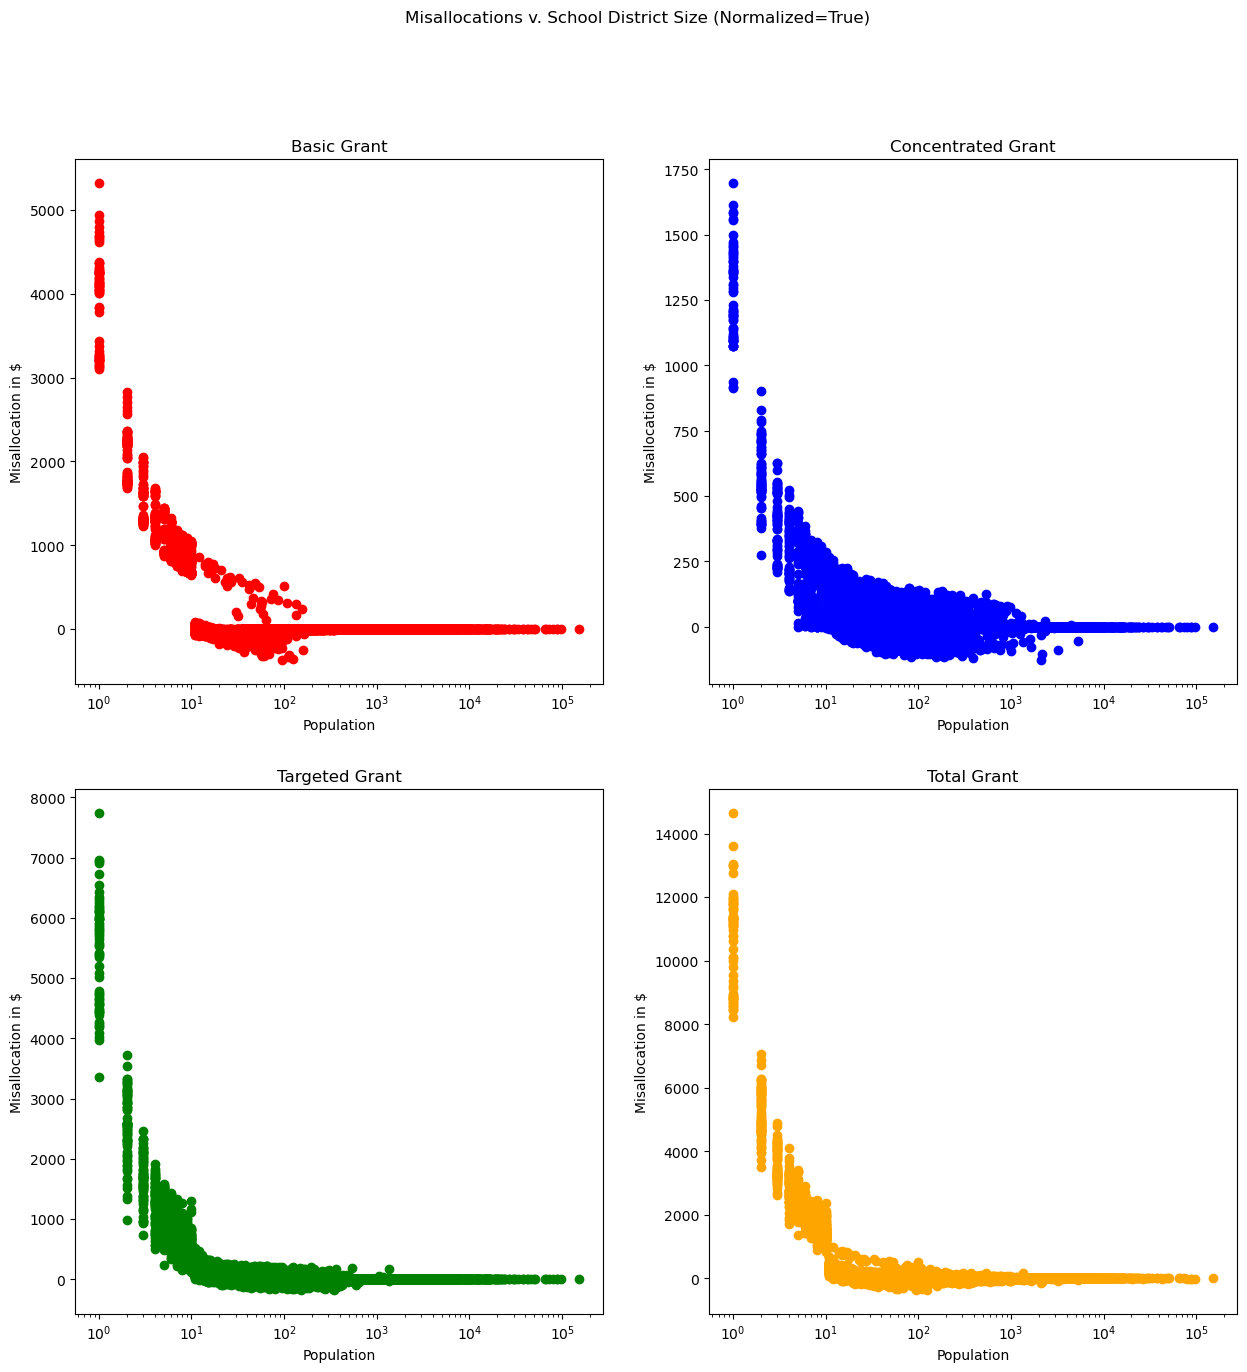
\includegraphics[width=0.7\linewidth]{images/all_grant_errors_normalized_vs_pop.png}
\caption{Disproportionate Title 1 Funds Allocations in the US}
\label{fig:missallocs_total}
\end{figure}


\begin{figure}[!ht]
    \centering
    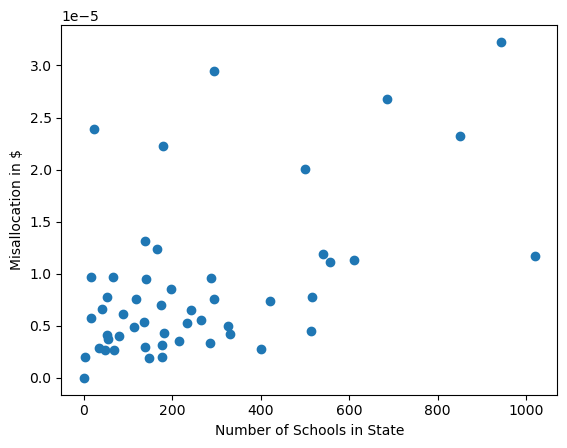
\includegraphics[width=0.48\linewidth, height=80pt]{images/af_vs_num_schools_per_state.png}
    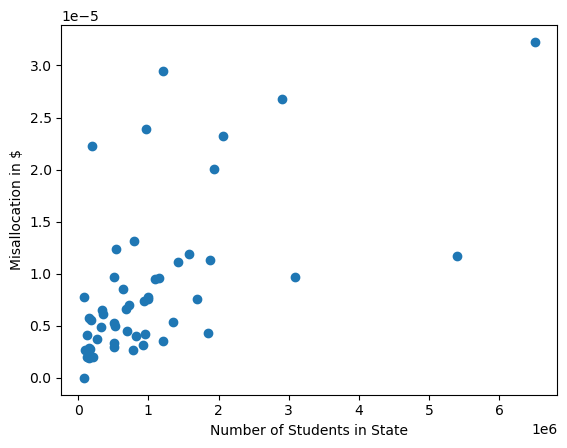
\includegraphics[width=0.48\linewidth, height=80pt]{images/af_vs_num_students_per_state.png}
    \caption{Correlation between number of schools (left) and number of students (right) per state with its level of $\alpha$ fairness. }
    \label{fig:corr_fair_num_schools}
    \label{fig:corr_fair_num_students}
\end{figure}


\begin{figure*}[h]
  \centering
  \begin{subfigure}[t]{0.49\linewidth}
    \centering
    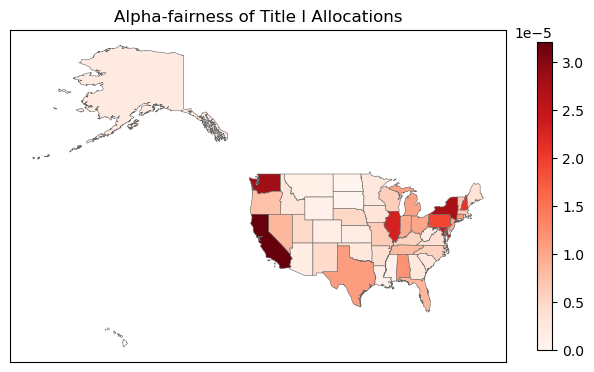
\includegraphics[width=\linewidth]{images/af_by_state.png}
    \caption{Level of $\alpha$ fairness per state under Baseline mechanism (BL) at $\rho = 2.56$}
    \label{fig:state_alpha}
  \end{subfigure}
  \hfill
  \begin{subfigure}[t]{0.49\linewidth}
    \centering
    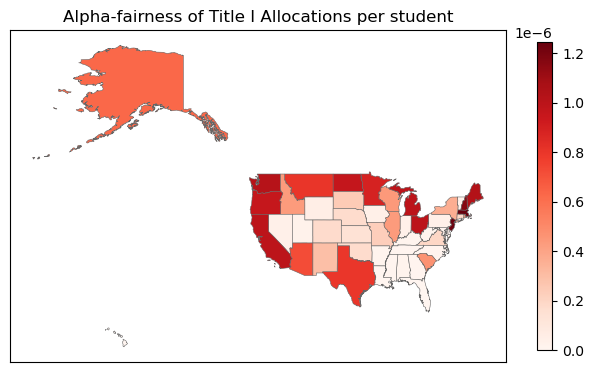
\includegraphics[width=\linewidth]{images/af_by_student.png}
    \caption{Level of $\alpha$ fairness per student under Baseline mechanism (BL) at $\rho = 2.56$}
    \label{fig:student_alpha}
  \end{subfigure}
  \caption{Fairness comparison}
  \label{fig:fairness_comparison}
\end{figure*}


\begin{figure*}[h]
\centering
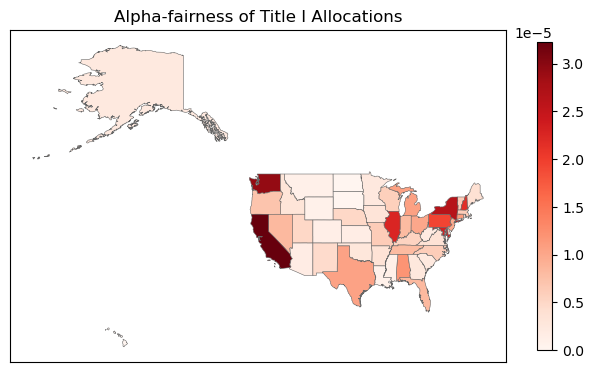
\includegraphics[width=0.5\linewidth]{images/af_states_map.png}
\caption{Level of  $\alpha$ fairness per state  under Baseline mechanism (BL) at $\rho = 2.56$}
\label{fig:state_alpha}
\end{figure*}



It can be seen from Figure \ref{fig:missallocs_total} that schools of low population receive far more money than they actually need as a consequence of the bias in the allocation mechanism, while larger districts may actually receive less funding. This figure made a clear evidence on the disparate impact of the privacy preserving mechanism in practice. 


\subsection*{Further analysis}

While there is a some level of unfairness under privacy-preserving mechanism towards different school districts,  we observed that level varies differently by state. We report the fairness level per state, i.e the difference between the maximum bias minus the minimum bias per state in Figure \ref{fig:state_alpha}. We see that under $\rho = 2.65$ California has the largest unfairness level over its schools.   

To understand why California has the highest  level of unfairness,  we provide the scatter plot between level of fairness $\alpha$ per state with its number of schools and its number of students in Figure \ref{fig:corr_fair_num_schools}. We observed a Pearson correlation of 0.37 between the number of schools per state and its fairness level. Also, a high Pearson correlation of 0.71 between number of state's students and its fairness level . A In other words, the state with more schools and more students tends to be suffered more unfairness. For example, the California state has the highest number of students, more than 6.5 million students overall. It also ranks secondly based on the number of schools with  1022 schools just below Texas with 1222 schools. This partly explains why this state suffers the most unfairness for all schools as showed in Figure \ref{fig:state_alpha}. 

\subsection*{Misallocations noramlized per student}
Examining both total misallocations and misallocations per student is crucial when assessing the impact of differential privacy on the allocation of Title I education funds in districts. Total misallocations provide a comprehensive perspective by considering the absolute magnitude of funding disparities across states. It enables us to identify states that are disproportionately affected in terms of the overall amount of misallocated funds. This analysis is important because significant total misallocations could lead to substantial disparities in educational resources, hindering the ability of disadvantaged districts to provide quality education.

On the other hand, evaluating misallocations per student offers a more nuanced understanding of the fairness of funding distribution. It allows us to account for the relative impact on individual students within each state. By examining misallocations per student, we can identify states where the disparity in funding affects a larger proportion of the student population, potentially exacerbating educational inequalities and limiting opportunities for marginalized students.

When funds are misallocated in total, it can particularly affect certain types of funding. For instance, if a state with a higher population of disadvantaged students experiences a significant total misallocation, it may receive insufficient funding to adequately support targeted interventions, such as specialized educational programs, additional resources, or support services for at-risk students. This can further perpetuate existing disparities and hinder efforts to address educational inequities.

Similarly, when funds are seen misallocated per student, it highlights the distributional challenges faced by specific states. If a state with a higher concentration of disadvantaged students experiences larger misallocations per student, it may imply that individual students in that state are being deprived of the financial support they require to succeed academically. This can impact the availability of resources such as instructional materials, qualified teachers, technology, or extracurricular activities, impeding their educational progress and perpetuating systemic inequalities.

In conclusion, analyzing both total misallocations and misallocations per student provides a comprehensive understanding of the impact of differential privacy on the allocation of Title I education funds. This dual perspective helps identify states disproportionately affected in terms of both the absolute amount of misallocated funds and the relative impact on individual students. By examining these two aspects, policymakers can gain insights into the specific challenges faced by different states and devise targeted strategies to ensure fair and equitable distribution of education funds.

\section*{Section 203 of the Voting Rights Act}
Section 203 of the Voting Rights Act requires certain jurisdictions to provide bilingual election materials and assistance to voters who are not proficient in English. To determine which jurisdictions are covered by this provision, the Census Bureau collects data on the number and percentage of voting-age citizens who are members of a language minority group and have limited English proficiency.

The Census Bureau uses three measures to calculate these numbers: the Limited English Proficient Population Count (LEPPCT), the Voting Age Citizen In-Language Count (VACIT), and the Voting Age Citizen Language Minority Group Citizen Voting Age Population (VACLEP).

The LEPPCT is the percentage of people in a language minority group who have limited English proficiency. The VACIT is the number of voting-age citizens who are members of a language minority group and who have indicated a need for language assistance in voting. The VACLEP is the number of voting-age citizens who are members of a language minority group.

By using these three measures, the Census Bureau determines which jurisdictions meet the criteria for coverage under Section 203. This information is then used by election officials to provide bilingual election materials and assistance to voters who need it, ensuring that everyone has an equal opportunity to participate in the electoral process.

\subsection*{Allocation Formula}
To explain how coverage is computed based on the given formulas, we can break them down into terms:
\begin{figure*}[h]
\centering
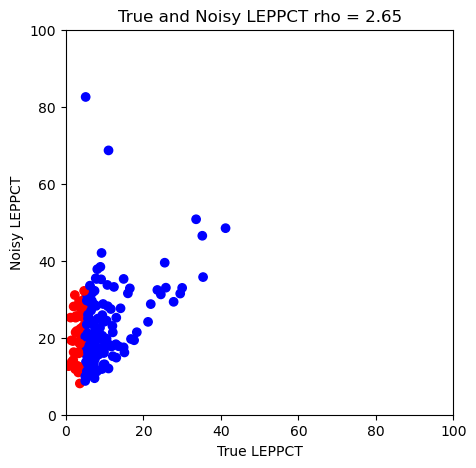
\includegraphics[width=0.5\linewidth]{images/true_noisy_leppct_2.65.png}
\caption{LEPPCT vs. LEPPCT noisy values after DP mechanism at $\rho=2.65$}
\label{fig:state_alpha}
\end{figure*}



\section*{Differentially Private mechanisms}
To release privately the outcomes $P^F_i$ given a privacy constraint $\epsilon$, there are several mechanisms. These mechanisms can roughly be divided into the two categories, strict and non-strict allocation mechanisms. A strict allocation mechanism requires that
its outcome should always lie in the probability simplex $\Delta_n = \{x \  | x \in {\mathbb{R}^{+}}^{n}, \boldsymbol{1}^T x =1 \}$ while a non-strict allocation mechanism
only asks its output to be non-negative. The rest of this report aims to study the (approximate) optimal
(strict allocation) mechanisms under different fairness metrics.
    \subsection*{Strict Allocation Mechanism}
    
    \begin{definition}[Baseline Mechanism (BL)]
        The \emph{baseline mechanism} outputs the allocation for each distribute $i\in [n]$ as follows.
        \begin{equation*}
            \blmech{\noisydata}_i = \frac{a_i\cdot \relu{\tilde{x}_i}}{\sum_{j=1}^n a_j\cdot \relu{\tilde{x}_j}}\,.
        \end{equation*}
    \end{definition}
    
Where $\tilde{x}_i$ is the noisy private population count, while the supscript $x_{+} = \max(x, 0)$ takes the non-negative part of the number $x$.


    \begin{definition}[Projection onto Simplex Mechanism (PoS)]
        The \emph{projection onto simplex mechanism} outputs the allocation for each distribute $i\in [n]$ as follows.
        \begin{equation*}
            \posmech{\noisydata}_i = \underset{\bm{v}\in\RR^n}{\arg\min}~\norm{\bm{v}-\noisyalloc}_2\qquad\mathrm{s.t.}~
            \sum_{i=1}^n v_i = 1,~\bm{v}\geq \bm{0}\,.
        \end{equation*}
    \end{definition}
    
    \subsection*{Non-strict Allocation Mechanism}
    \begin{definition}[Positive Allocation Mechanism (PA)]
        The \emph{positive allocation mechanism} 
        outputs the allocation for each distribute $i\in [n]$ as follows.
        \begin{equation*}
            \pamech{\noisydata}_i  =  \relu{\nalloci{i}}= \relu{\frac{a_i\cdot \tilde{x}_i}{\sum_{j=1}^n a_j\cdot \tilde{x}_j}}\,.
        \end{equation*}
    \end{definition}
    \begin{definition}[Repair Mechanism (RP) \cite{pujol2020fair}]
        The \emph{repair mechanism} outputs the allocation for each distribute $i\in [n]$ as follows.
        \begin{equation*}
            \rpmech{\noisydata}_i  = \frac{a_i\cdot \relu{\tilde{x}_i}+\Delta}{\sum_{j=1}^n a_j\cdot \relu{\tilde{x}_j} - \Delta'}\,,
        \end{equation*}
        where 
        \begin{equation*}
            \Delta= \frac{\ln\left(2n/\delta\right)}{\epsilon}\,,\qquad\Delta' = 
            \frac{n\ln\left(2n^2/\delta\right)}{\epsilon}\,.
        \end{equation*}
    \end{definition}
    
    \begin{proposition}[No-penalty allocation \cite{pujol2020fair}]
        The following inequality holds with probability at least $1-\delta$.
        \begin{equation*}
            \rpmech{\noisydata}_i\geq \talloci{i}\,,\qquad\forall~i\in[n]\,.
        \end{equation*}
    \end{proposition}


\section*{Source of unfairness}
We investigate the two main sources of unfairness highlighted in previous section: (1) shape of allocation function and (2) post-processing steps. 
\subsection*{Shape of allocation function}

\begin{theorem}
\label{lem:fair_bound_allottments}
Let $P$ be an allotment problem which is at least twice differentiable.
A data-release mechanism $\cM$ is $\alpha$-fair w.r.t.~$P$ for some 
$\alpha < \infty$ if there exist some constant values 
% $c_i \; (i \in [n])$ such that,
% for all datasets $\bm{x} \in \cX$, 
% \[
% \Tr(\bm{H}P_i)(\bm{x}) = c_i \;\; (i \in [n]).
% \]
$c^i_{jl} \; (i \in [n], j,l \in [k])$ such that, for all datasets $\bm{x} \in \cX$, 
\[
  (\bm{H}P_i)_{j,l}(\bm{x}) = c^i_{j,l}   \;\; (i\in[n]\; j,l\in[k]).
\]
\end{theorem}

\begin{corollary}
\label{cor:2}
If $P$ is a linear function, then $\cM$ is fair w.r.t.~$P$.
\end{corollary}


\begin{corollary}
\label{cor:3}
$\cM$ is fair w.r.t.~$P$ if there exists a constant $c$ such that,
for all dataset $\bm{x}$, 
\[
\mbox{Tr}(\bm{H}P_i)(\bm{x}) = c \;\; (i \in [n]).
\]
\end{corollary}

\begin{corollary}
Consider an allocation problem $P$. Mechanism $\cM$ is not fair
w.r.t.~$P$ if there exist two entries $i, j \in [n]$ such that
$\mbox{Tr}(\bm{H}P_i)(\bm{x}) \neq \mbox{Tr}(\bm{H}P_j)(\bm{x})$ for some dataset
$\bm{x}$.
\end{corollary}

\noindent
The above implies that fairness cannot be achieved if $P$ is \emph{a
  non-convex function}, as is the case for \emph{all} the allocation
problems considered in this paper. {\em A fundamental consequence of
  this result is the recognition that adding Laplacian noise to the
  inputs of the motivating example will necessarily introduce fairness
  issues.} For instance, consider $\tfa$ and notice that the trace of
its Hessian
\[
\mbox{Tr}(\bm{H}\tfa_i) = 2a_i \left[
\frac{x_i \sum_{j\in[n]} a_j^2 - a_i \left(\sum_{j\in[n]} x_ja_j\right)}
     {\left(\sum_{j\in[n]}x_ja_j\right)^3}
\right],
\]
is not constant with respect to its inputs. Thus, any two entries $i,
j$ whose $x_i \neq x_j$ imply $\mbox{Tr}(\bm{H}\tfa_i) \neq
\mbox{Tr}(\bm{H}\tfa_j)$.  As illustrated in Figure \ref{fig:p1motivation},
Problem $\tfa$ can introduce significant disparity errors.  For $\epsilon = 0.001,
0.01$, and $0.1$ the estimated fairness bounds are $0.003$, $3\times
10^{-5}$, and $1.2\times 10^{-6}$ respectively, which amount to an
average misallocation of \$43,281, \$4,328, and \$865.6 respectively.
The estimated fairness bounds were obtained by performing a linear
search over all $n$ school districts and selecting the maximal
$\mbox{Tr}(\bm{H}\tfa_i)$.


\subsection*{Impact of post-processing}
The post-processing steps can be applied at the inputs $x$, over the outcome $P^F_{i}(x)$ or at both. We investigate the impact of post-processing over input and outcome separately in this section.


\subsubsection*{Post-processing over the inputs}
This step is performed to make sure the released private counts satisfies consistency constraints \cite{cohen2021census}. For example, the released private counts should be non-negative integer numbers, or sum of counts at all cities' in a state should be equal to that state's count. 


\noindent \textbf{Non-negative truncation} $\tilde{x} = \max(0, \tilde{x}) $

We have the following result which state that non-negative truncation introduces positive bias, and the closer to zero the true count is, the higher the bias. 
\begin{theorem}
  \label{lem:exp_clipped_lap}
  Let $\tilde{x} = x + \mbox{Lap}(\lambda)$, with scale $\lambda > 0$, 
  and $\hat{x} = \text{PP}^{\geq \ell}(\tilde{x})$, with $\ell < x$, 
  be its post-processed value. Then, 
  $$ 
    \EE[\hat{x}] = x + \frac{\lambda}{2} \exp(\frac{\ell - x}{\lambda} ).
  $$
\end{theorem}


\noindent \textbf{Integral transform} 

The integral transform $\text{PP}^{\mathbb{N}}(z)$ is used when the released data should be of integral quantities. To make sure that this processing step does not introduce additional bias, we can rely on the stochastic rounding technique:

\begin{equation}
    \text{PP}^{\mathbb{N}}(z) = \begin{cases} \lfloor z \rfloor   \ \mbox{w.p.:} \  1 -(z- \lfloor z \rfloor ) \\
                               \lfloor z \rfloor  +1 \ \ \mbox{w.p.:} \  z - \lfloor z \rfloor 
    \end{cases}
\end{equation}


The stochastic rounding guarantees  that $\mathbb{E} [\text{PP}^{\mathbb{N}}(\tilde{x})] = \tilde{x} $ so no additional bias will introduce to $\text{PP}^{\mathbb{N}}(\tilde{x})$


\subsubsection*{Post-processing over the outcomes}

\section*{Mitigating Solutions}
\subsection*{Mechanisms}
    Different kind of post-processing mechanisms are considered in this section. These mechanisms
    require that
    their outcomes should always lie in the probability simplex $\Delta_n$. The rest of this work aims to study the (approximate) optimal mechanisms under different fairness metrics.
    \begin{definition}[Baseline Mechanism (BL)]
        The \emph{baseline mechanism} outputs the allocation for each entity $i\in [n]$ as follows.
        \begin{equation*}
            \cM_{\mathrm{BL}}(\noisydata)_i = \frac{a_i\cdot \relu{\tilde{x}_i}}{\sum_{j=1}^n a_j\cdot \relu{\tilde{x}_j}}\,.
        \end{equation*}
    \end{definition}
    
    \begin{definition}[Projection onto Simplex Mechanism (PoS)]
        The \emph{projection onto simplex mechanism} outputs the allocation for each entity $i\in [n]$ as follows.
        \begin{equation*}
            \cM_{\mathrm{PoS}}(\noisydata)_i= \underset{\bm{v}\in\RR^n}{\arg\min}~\norm{\bm{v}-\noisyalloc}_2\qquad\mathrm{s.t.}~
            \sum_{i=1}^n v_i = 1,~\bm{v}\geq \bm{0}\,.
        \end{equation*}
    \end{definition}


% \bibliographystyle{acm}  
%  \bibliography{lib.bib}
%\bibliography{lib.bib}
\end{document}
